\documentclass[12pt,a4paper]{article}

\usepackage[T1]{fontenc}
\usepackage[utf8]{inputenc}
\usepackage{lmodern}
\usepackage[margin=1in]{geometry}
\usepackage{setspace}
\usepackage{hyperref}
\usepackage{booktabs}
\usepackage{longtable}
\usepackage{array}
\usepackage{graphicx}
\usepackage{float}
\usepackage{xcolor}
\usepackage{listings}
\usepackage{enumitem}
\usepackage{titlesec}

\hypersetup{
  colorlinks=true,
  linkcolor=blue,
  urlcolor=blue,
  citecolor=blue,
  pdftitle={Detecting Data Leaks via SQL Injection: AWS Project Report},
  pdfauthor={Cloud Computing Project Team}
}

\setstretch{1.2}
\setlist[itemize]{leftmargin=1.5em}
\setlist[enumerate]{leftmargin=1.8em}

\titleformat{\section}{\large\bfseries}{\thesection}{0.7em}{}
\titleformat{\subsection}{\normalsize\bfseries}{\thesubsection}{0.6em}{}

\lstdefinestyle{bashstyle}{
  basicstyle=\ttfamily\small,
  breaklines=true,
  frame=single,
  backgroundcolor=\color{gray!8},
  columns=fullflexible
}

\title{Detecting Data Leaks via SQL Injection in AWS\\[0.25em]
\large Professional Technical Report}
\author{Cloud Computing Project Team}
\date{April 19, 2026}

\begin{document}

\maketitle
\tableofcontents
\newpage

\section{Abstract}
This report presents the design, implementation, and evaluation of a cloud-native security pipeline for SQL injection (SQLi) attacks in Amazon Web Services (AWS). The project intentionally deploys a vulnerable Flask application backed by Amazon RDS MySQL, then measures how effectively layered cloud controls detect and mitigate data exfiltration attempts. The implementation combines AWS WAF, API Gateway, Kinesis, Lambda, CloudWatch, SNS, and S3 to create an end-to-end detection and response flow. Three SQLi attack classes were executed: union-based, boolean-based blind, and error-based attacks. Results show that direct data leakage is possible without defenses, while managed and custom WAF controls substantially reduce exploit success. The report documents payloads, observed outcomes, leaked data fields, and operational constraints such as rate-limit evaluation windows. It also maps risks through STRIDE and proposes hardening actions, including parameterized queries, improved WAF custom signatures, and continuous detection tuning.

\section{Introduction}
SQL injection remains one of the most impactful application security weaknesses because it targets the core trust boundary between user-controlled input and backend database queries. In this project, the team built a realistic AWS pipeline to show how SQLi attacks can be launched, detected, blocked, logged, and surfaced to operators. The architecture is intentionally layered so that each control addresses different portions of the kill chain:
\begin{itemize}
  \item Network and application edge filtering (API Gateway + WAF).
  \item Behavioral detection and classification (Lambda regex engine).
  \item Alerting and observability (SNS + CloudWatch dashboard).
  \item Forensic persistence (Kinesis + S3 archival).
\end{itemize}

The objective is not only to demonstrate exploitation, but to measure defense effectiveness and identify residual risk. The report therefore emphasizes evidence-driven comparisons between pre-WAF and post-WAF behavior and highlights where managed-rule signatures can still be evaded.

\section{Background: SQL Injection and Cloud Security}
\subsection{What SQL Injection Is}
SQL injection is a vulnerability class in which attacker-controlled input is interpreted as part of a database query rather than as inert data. When an application constructs SQL statements by concatenating raw input, attackers can alter query logic, bypass authentication, enumerate schema metadata, or extract sensitive records. SQLi can impact confidentiality, integrity, and availability in a single technique family.

In the tested application, vulnerable endpoints accepted query parameters and interpolated them into SQL statements. This allowed both authentication bypass attempts and data extraction attempts against user records.

\subsection{Why SQL Injection Happens}
From a secure coding perspective, SQLi is a failure of input handling and query construction discipline. Typical root causes include:
\begin{itemize}
  \item Unsanitized user input reaching query builders.
  \item Direct string concatenation for SQL statements.
  \item Lack of prepared statements and parameter binding.
  \item Over-privileged database accounts that expand blast radius.
  \item Missing input validation and weak output/error handling.
\end{itemize}

Even if an application hides SQL errors from users, attackers can still use inferential techniques such as boolean-blind injection and time-based probing to reconstruct data. Therefore, secure design must address both obvious and subtle leakage paths.

\subsection{OWASP Context}
SQL injection remains a foundational issue within modern application security risk models and is strongly aligned with the OWASP Top 10 category focused on injection flaws. OWASP rankings evolve over editions, but injection-related weakness categories continue to represent high-likelihood and high-impact risks because of their direct path to sensitive data compromise. In cloud environments, SQLi can be amplified by misconfigured identity permissions, centralized data stores, and internet-exposed APIs.

\subsection{Real-World Relevance}
Historically, major incidents involving large-scale data exposure have included injection-style weaknesses or adjacent input-validation failures. Common lessons from widely discussed breaches include:
\begin{itemize}
  \item Public-facing endpoints frequently become initial access points.
  \item Attackers pivot from one vulnerable query to broad data access.
  \item Weak logging and delayed detection increase dwell time.
  \item Compliance and reputational damage often exceed immediate technical loss.
\end{itemize}

The practical takeaway is that SQLi defense must be multi-layered: secure code, preventive edge controls, runtime detection, and strong operational response.

\section{System Architecture and Setup}
\subsection{Deployment Topology}
The project architecture follows a five-layer model: attack simulation, network defense, detection engine, logging pipeline, and alerting/dashboard. The core traffic path is:
\begin{center}
Attacker $\rightarrow$ API Gateway $\rightarrow$ WAF $\rightarrow$ Flask App (EC2) $\rightarrow$ RDS MySQL
\end{center}

In parallel, telemetry is streamed to Kinesis and Lambda for analysis, then persisted in DynamoDB/S3 and visualized via CloudWatch and a frontend dashboard.

\subsection{Environment Details}
\begin{itemize}
  \item Target host: 3.144.240.191 (Flask app on port 5000).
  \item Attacker host: 18.221.229.40.
  \item Database: Amazon RDS MySQL, database name \texttt{userdata}.
  \item Vulnerable endpoints: \texttt{/login} and \texttt{/search}.
  \item API endpoint used in defense tests: \url{https://2y68q1dt27.execute-api.us-east-2.amazonaws.com/prod}.
\end{itemize}

\subsection{Detection and Logging Components}
The Lambda detector uses regex-based pattern classification with severities (LOW, MEDIUM, HIGH, CRITICAL) and writes findings to DynamoDB. High-severity events trigger SNS notifications. Firehose/Kinesis settings use buffered delivery to S3, enabling historical investigation and long-term retention policies.

\section{Threat Model (STRIDE Framework)}
\begin{table}[H]
\centering
\caption{STRIDE Threat Mapping for This Project}
\begin{tabular}{p{0.2\textwidth} p{0.25\textwidth} p{0.47\textwidth}}
\toprule
\textbf{STRIDE Category} & \textbf{Threat Focus} & \textbf{Example in This Project} \\
\midrule
Spoofing & Identity impersonation & Attacker attempts login bypass using SQLi patterns to authenticate as privileged user. \\
Tampering & Data integrity compromise & Injection payloads could execute unauthorized updates/deletes if write queries are reachable. \\
Repudiation & Non-repudiation failure & Without reliable audit logs, attackers can deny malicious requests. \\
Information Disclosure & Confidentiality breach & UNION-based extraction leaks sensitive columns such as full name, email, SSN, and credit card. \\
Denial of Service & Availability degradation & Time-delay or heavy-query payloads (for example sleep-based probes) increase latency and can exhaust resources. \\
Elevation of Privilege & Access control bypass & Metadata enumeration (for example information\_schema) helps attackers discover additional tables and privileges. \\
\bottomrule
\end{tabular}
\end{table}

\section{Implementation: Attack Simulation (Section 4)}
\subsection{Testing Methodology}
Attack simulation combined automated SQLMap campaigns and manual payload tests. SQLMap was selected to ensure repeatability across techniques while manual URLs were used to validate edge behaviors and direct endpoint responses.

The three attack classes executed were:
\begin{enumerate}
  \item Union-based SQL injection.
  \item Boolean-based blind SQL injection.
  \item Error-based SQL injection.
\end{enumerate}

\subsection{Exact Attack Commands (SQLMap)}
\begin{lstlisting}[style=bashstyle,caption={Union-based SQLi command}]
python3 sqlmap.py -u "http://3.144.240.191:5000/search?name=test" --technique=U --dbs --dump --batch -v 3
\end{lstlisting}

\begin{lstlisting}[style=bashstyle,caption={Boolean-based blind SQLi command}]
python3 sqlmap.py -u "http://3.144.240.191:5000/login?username=admin&password=test" --technique=B -D userdata -T users --dump --batch -v 2
\end{lstlisting}

\begin{lstlisting}[style=bashstyle,caption={Error-based SQLi command}]
python3 sqlmap.py -u "http://3.144.240.191:5000/login?username=admin&password=test" --technique=E --dump-all --batch
\end{lstlisting}

\subsection{Exact Manual Payload URLs Used}
\begin{longtable}{p{0.25\textwidth} p{0.68\textwidth}}
\caption{Manual Attack URLs Recorded in the Lab}\\
\toprule
\textbf{Attack Case} & \textbf{Payload / URL} \\
\midrule
\endfirsthead
\toprule
\textbf{Attack Case} & \textbf{Payload / URL} \\
\midrule
\endhead
Login bypass test & \url{http://3.144.240.191:5000/login?username=admin%27--&password=x} \\
UNION extraction test & \url{http://3.144.240.191:5000/search?name=%27%20UNION%20SELECT%20id,full_name,ssn%20FROM%20users--} \\
Table enumeration test & \url{http://3.144.240.191:5000/search?name=%27%20UNION%20SELECT%201,table_name,3%20FROM%20information_schema.tables--} \\
Time delay test & \url{http://3.144.240.191:5000/login?username=admin%27%20AND%20SLEEP(5)--&password=x} \\
\bottomrule
\end{longtable}

\subsection{Leaked Data and Exposure Scope}
Across successful pre-defense runs, the following high-risk fields were reported as exposed:
\begin{itemize}
  \item full\_name
  \item email
  \item ssn
  \item credit\_card
  \item dob
\end{itemize}

From a compliance perspective, SSN and payment-related fields indicate direct personally identifiable information (PII) and potential financial-data exposure.

\subsection{Result Comparison by Attack Type}
\begin{longtable}{p{0.2\textwidth} p{0.19\textwidth} p{0.18\textwidth} p{0.18\textwidth} p{0.18\textwidth}}
\caption{Attack Results, Timing, and WAF Outcome Matrix}\\
\toprule
\textbf{Attack Type} & \textbf{Payload Pattern} & \textbf{Data Leak (No WAF)} & \textbf{Approx. Time Taken} & \textbf{Blocked by WAF?} \\
\midrule
\endfirsthead
\toprule
\textbf{Attack Type} & \textbf{Payload Pattern} & \textbf{Data Leak (No WAF)} & \textbf{Approx. Time Taken} & \textbf{Blocked by WAF?} \\
\midrule
\endhead
Union-based & UNION SELECT & Yes: user records including PII fields & Placeholder: capture from SQLMap summary screen & Yes, by AWSManagedRulesSQLiRuleSet \\
Boolean blind & true/false inference & Yes: inferred user data & Placeholder: capture from SQLMap summary screen & Yes, via custom rate limit behavior \\
Error-based & DB error exploitation & Yes: table and schema details & Placeholder: capture from SQLMap summary screen & Partially mitigated by managed rules; verify with screenshots \\
Time-delay probe & SLEEP(5) & No direct row dump, but service latency impact observed & 5 seconds in manual test endpoint response & Yes, by AWSManagedRulesKnownBadInputs \\
\bottomrule
\end{longtable}

\subsection{WAF Effectiveness and Residual Risk}
Defense testing showed strong improvement after WAF controls were enabled:
\begin{itemize}
  \item UNION SELECT payloads moved from data leakage to explicit blocking.
  \item Always-true payloads with OR 1=1 were blocked by SQLi rule sets.
  \item Time-delay signatures were blocked by known-bad-inputs coverage.
\end{itemize}

However, testing also exposed two operational caveats:
\begin{enumerate}
  \item A minimal payload such as \texttt{admin'--} could evade managed signatures when no common SQL keyword token was present.
  \item Custom rate limits were not instantaneous and appeared to apply over AWS evaluation windows (roughly 30 to 60 seconds), creating a short burst window before enforcement.
\end{enumerate}

These findings emphasize that managed WAF rules are necessary but not sufficient. They should be augmented with custom signatures and application-layer hardening.

\subsection{Required Screenshot Placeholders for Final Submission}
\begin{figure}[H]
\centering
\IfFileExists{figures/figure-a-sqlmap-output.png}{
  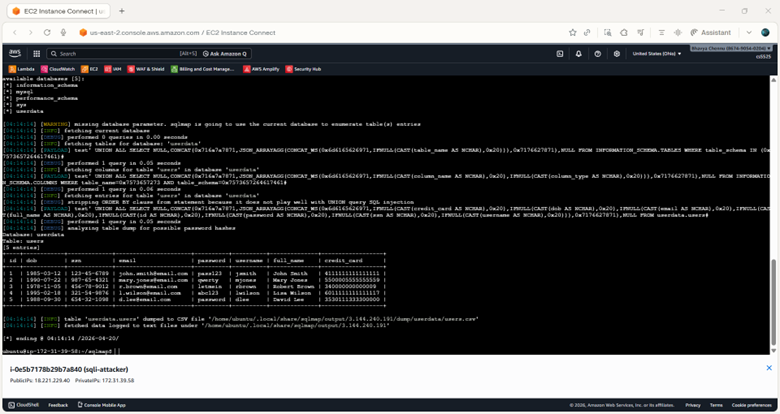
\includegraphics[width=0.96\textwidth]{figures/figure-a-sqlmap-output.png}
}{
  \fbox{\parbox{0.9\textwidth}{\textbf{Placeholder Figure A:} SQLMap union-based extraction terminal output showing extracted columns and total runtime.}}
}
\caption{Figure A. SQLMap extraction output from the attack simulation environment}
\end{figure}

\begin{figure}[H]
\centering
\IfFileExists{figures/figure-b-waf-403.png}{
  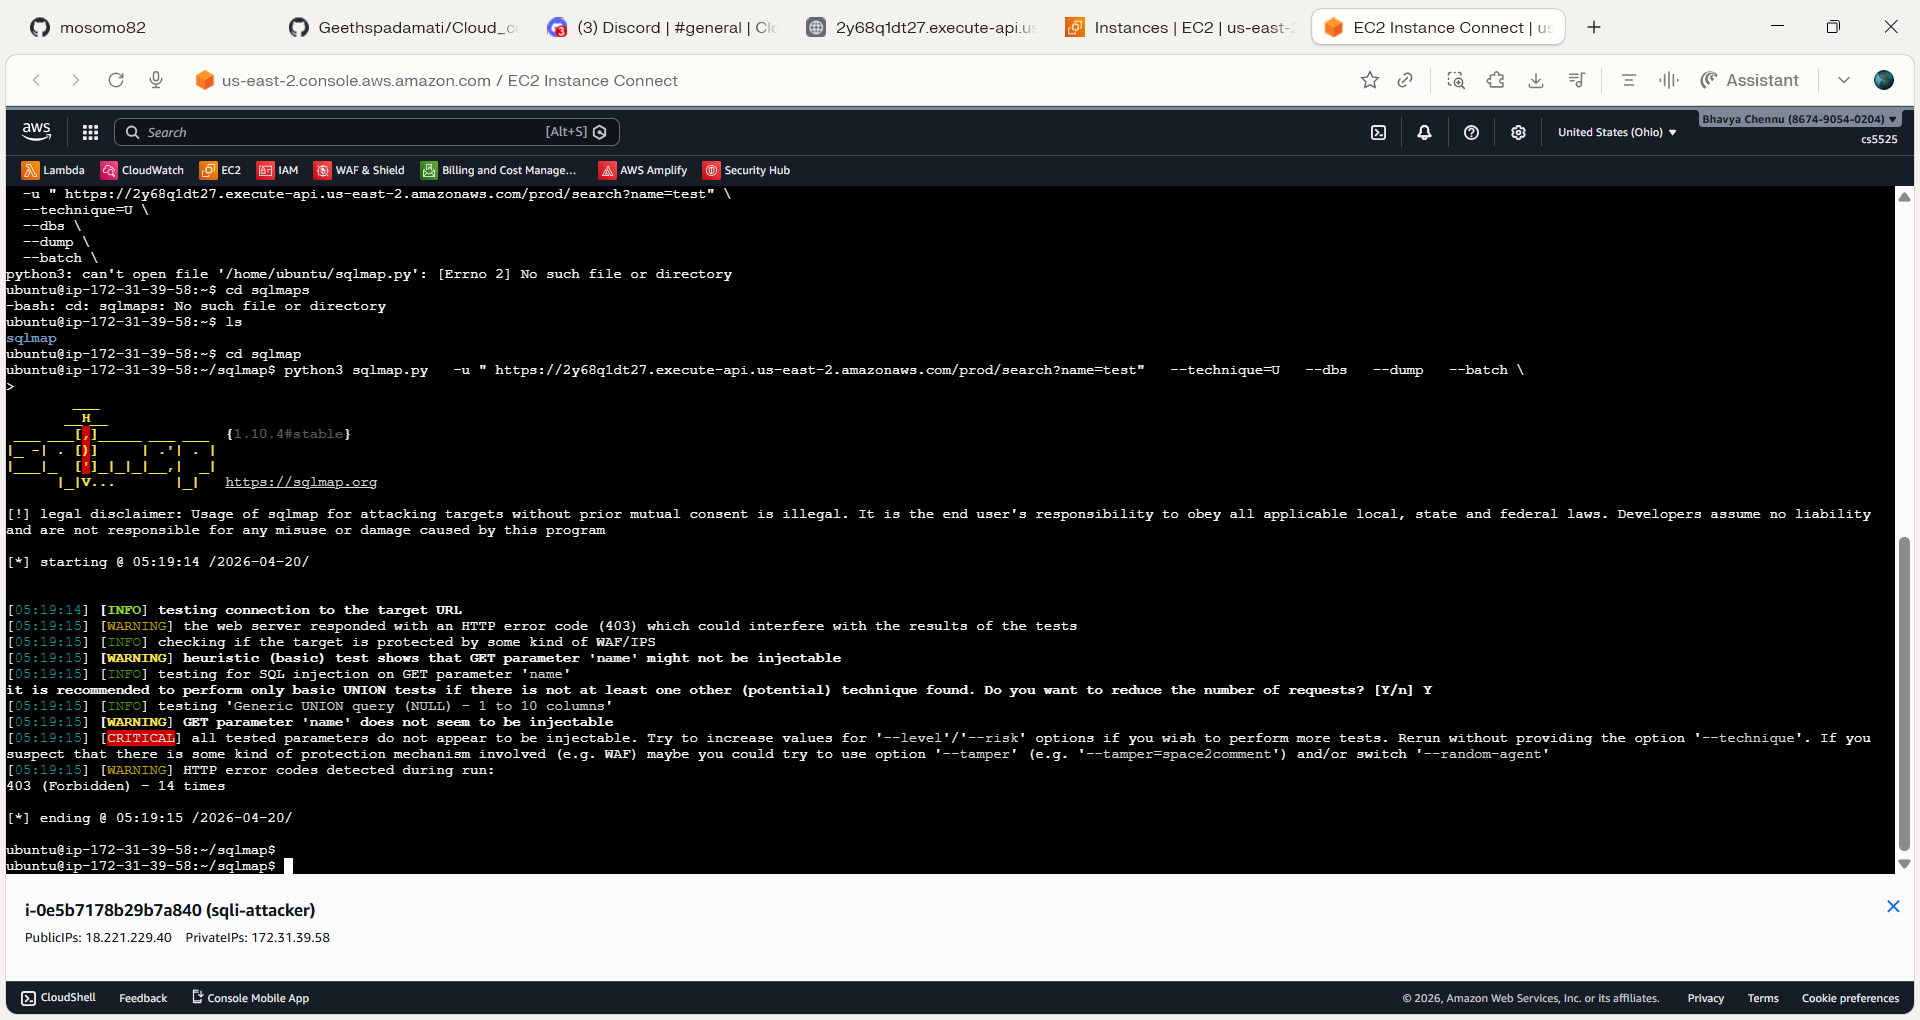
\includegraphics[width=0.96\textwidth]{figures/figure-b-waf-403.png}
}{
  \fbox{\parbox{0.9\textwidth}{\textbf{Placeholder Figure B:} Browser/API response showing WAF 403 block for blocked SQLi payload.}}
}
\caption{Figure B. WAF 403 Forbidden block response during SQLi payload test}
\end{figure}

\begin{figure}[H]
\centering
\IfFileExists{figures/figure-c-dashboard-live.png}{
  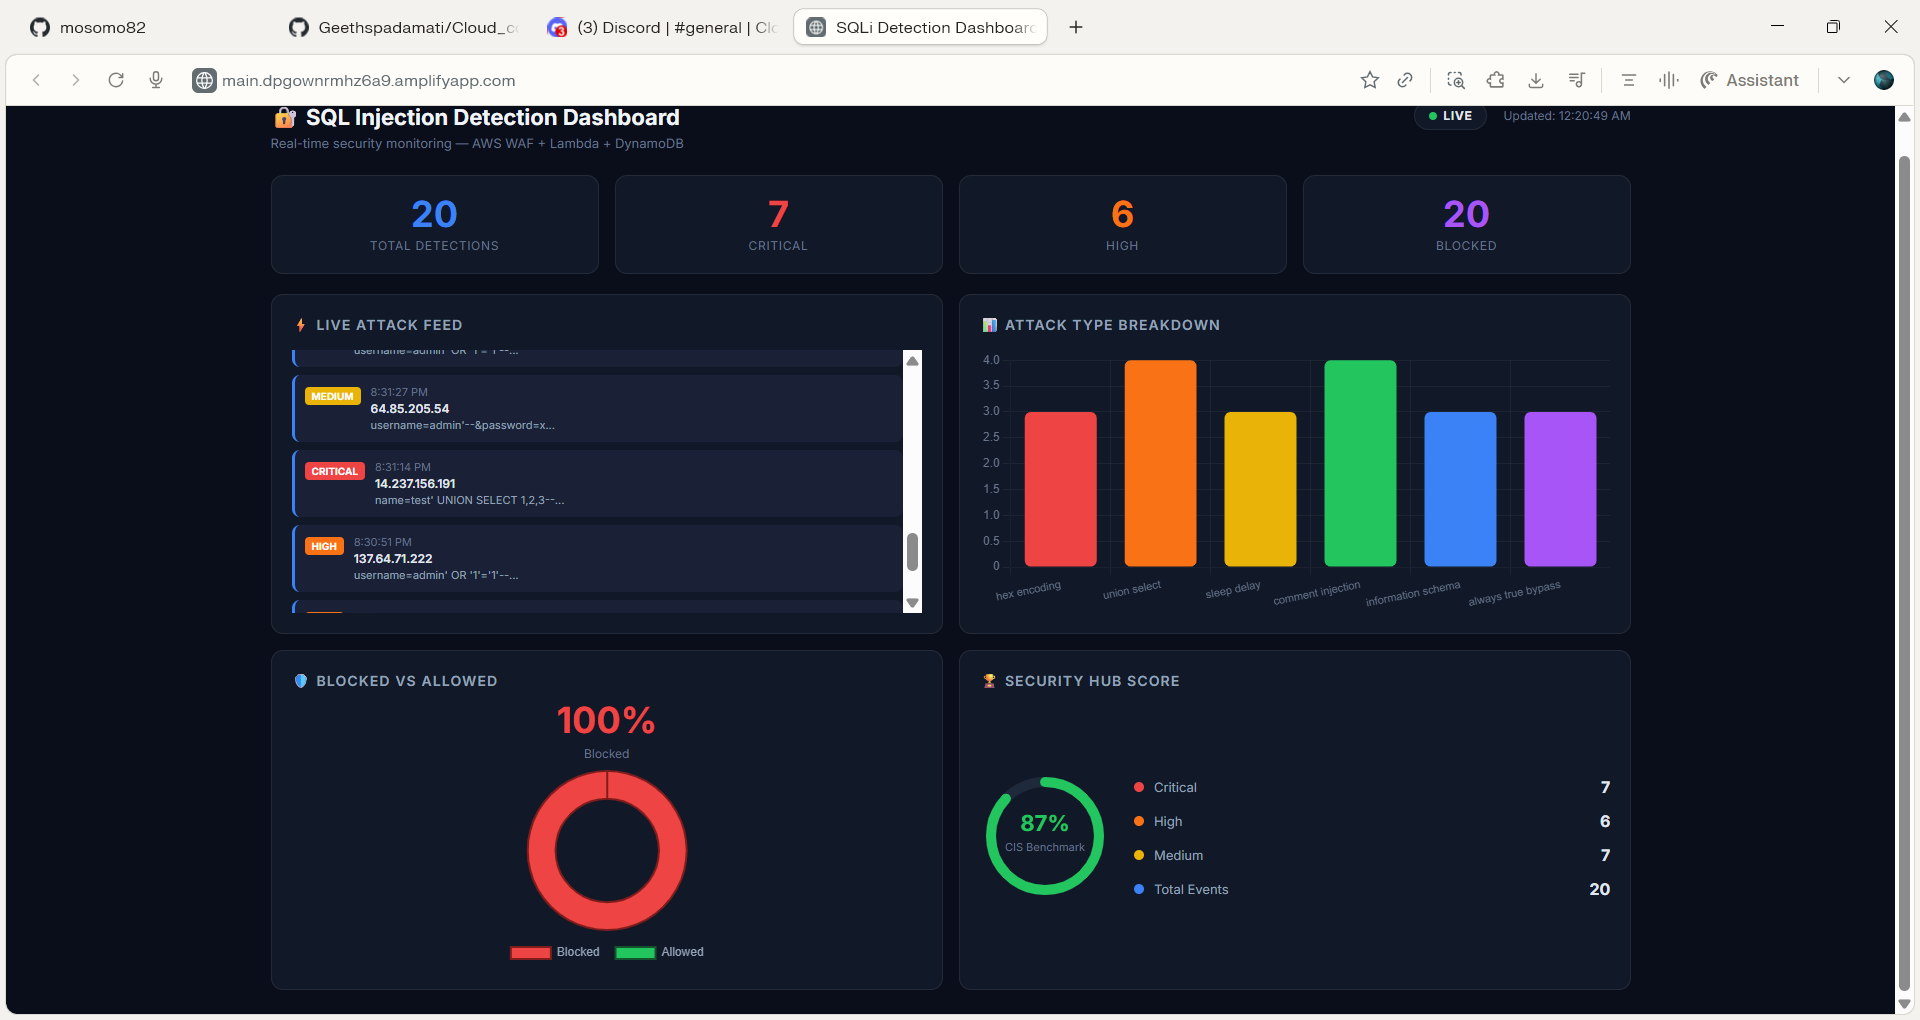
\includegraphics[width=0.96\textwidth]{figures/figure-c-dashboard-live.png}
}{
  \fbox{\parbox{0.9\textwidth}{\textbf{Placeholder Figure C:} Dashboard/CloudWatch panel during attack run showing blocked and detected counts.}}
}
\caption{Figure C. CloudWatch security dashboard during active attack simulation}
\end{figure}

\section{WAF and Network Defense Analysis}
\subsection{Controls Implemented}
Network defense centered on API Gateway fronting and AWS WAF managed rule groups with custom rate limiting. Key observed controls included SQLi-focused managed rules and bad-input signatures.

\subsection{Before/After Comparison}
\begin{table}[H]
\centering
\caption{Observed WAF Comparison Results}
\begin{tabular}{p{0.27\textwidth} p{0.2\textwidth} p{0.2\textwidth} p{0.26\textwidth}}
\toprule
\textbf{Attack Type} & \textbf{Without WAF} & \textbf{With WAF} & \textbf{Rule/Behavior} \\
\midrule
UNION SELECT & Leaked data & Blocked & AWSManagedRulesSQLiRuleSet \\
Always true OR 1=1 & Login bypassed & Blocked & AWSManagedRulesSQLiRuleSet \\
Boolean blind burst & Leaked data & Blocked after thresholding & Custom rate-limit rule \\
SLEEP() time delay & 5-second delay observed & Blocked & AWSManagedRulesKnownBadInputs \\
Normal request & Allowed & Allowed & Expected allow behavior \\
\bottomrule
\end{tabular}
\end{table}

\section{Detection Engine and Alerting Pipeline}
\subsection{Lambda Detection Logic}
The Lambda function classifies incoming request traces with regex rules mapped to severities. Examples include \texttt{union\_select} and \texttt{information\_schema} at CRITICAL severity, and \texttt{sleep\_delay} at HIGH severity. Findings are persisted to DynamoDB and high-severity findings are published to SNS.

This produces two operational advantages:
\begin{itemize}
  \item Fast triage through severity labels.
  \item Longitudinal visibility through structured finding records.
\end{itemize}

\subsection{Logging and Retention}
Firehose/Kinesis settings provide buffered log delivery to S3 partitions by date. Lifecycle policy then transitions storage classes over time and expires old objects, balancing forensic value and storage cost.

\section{Discussion}
The project demonstrates that SQLi remains practical against insecure query construction, especially in lab environments intentionally designed for educational exploitation. The key result is that defense-in-depth meaningfully changes outcomes: successful pre-defense exfiltration becomes largely blocked post-defense, while detection and alerting reduce mean time to awareness.

At the same time, edge-case bypass behavior highlights an important lesson. Security controls built on pattern signatures can miss low-context payloads, and timing-based controls may introduce delayed enforcement windows. Consequently, secure coding remains the primary control and WAF should be treated as a protective layer rather than a substitute for parameterized queries.

\section{Conclusion and Recommendations}
\subsection{Conclusion}
This implementation achieved an end-to-end cloud security workflow for SQL injection: simulate attacks, observe impact, apply controls, monitor outcomes, and document residual risk. The architecture successfully integrated preventive, detective, and response mechanisms across AWS services.

\subsection{Recommendations}
\begin{enumerate}
  \item Refactor application queries to use prepared statements and parameter binding everywhere.
  \item Add targeted custom WAF signatures to catch short evasive payloads such as comment-only bypass attempts.
  \item Expand automated regression tests to include both exploit payloads and false-positive controls.
  \item Track detection quality metrics explicitly: precision, recall, and alert latency.
  \item Preserve immutable evidence artifacts (screenshots, command output, response logs) for every test case in the final report package.
\end{enumerate}

\section*{Appendix A: Submission Checklist}
\begin{itemize}
  \item Exact payload/URL table included.
  \item Screenshot placeholders included and labeled for replacement.
  \item Leaked data fields listed: full\_name, email, ssn, credit\_card.
  \item Attack duration column included (replace placeholders with SQLMap terminal timings).
  \item WAF blocked/not-blocked outcomes documented per attack type.
\end{itemize}

\section*{Appendix B: Reference Artifacts Used}
\begin{itemize}
  \item attack-simulation/docs/attack-playbook.md
  \item attack-simulation/results/attack-summary.md
  \item defense/results/waf-comparison-results.md
  \item detection/lambda/handler.py
  \item infrastructure/cloudwatch.tf
  \item infrastructure/kinesis.tf
  \item infrastructure/s3.tf
  \item README.md
\end{itemize}

\end{document}
